\chapter{??????? ??????? ????????? ???????????? ????}\label{app:A}

??? ??????? ????????? ???? ??? ???????. ?????? ????????, ?? ? ??? ????? ????
???????? ? ?????????? ????????? (? ??? ????? ??????????? ?~????????????
?~?????????? ??????????), ?? ??????????? ?? ????????~\cref{lst:hwbeauty}.
\begin{ListingEnv}[!h]% ????????? floating ?????????? ????????? figure
    \captiondelim{ } % ??????????? ?????????????? ? ??????? ?? ????????????
    \caption{????????? ,,Hello, world`` ?? \protect\cpp}\label{lst:hwbeauty}
    % ????????? ????????? ??????? ? ????????? ? ????????? ?? ? ?????????? ? ???????????
    \begin{lstlisting}[language={[ISO]C++}]
	#include <iostream>
	using namespace std;

	int main() //????????? ? ???????????? ??? xelatex ? lualatex ????? ???????? ? ?????????
	{
		cout << "Hello, world" << endl; //latin letters in commentaries
		system("pause");
		return 0;
	}
    \end{lstlisting}
\end{ListingEnv}%
?????? ??~????? ????????, ?? ??? ??????????? (??.~???????~\cref{lst:hwplain}).
\begin{ListingEnv}[!h]
    \captiondelim{ } % ??????????? ?????????????? ? ??????? ?? ????????????
    \caption{????????? ,,Hello, world`` ??? ?????????}\label{lst:hwplain}
    \begin{Verb}

        #include <iostream>
        using namespace std;

        int main() //????????? ? ????????????
        {
            cout << "??????, ???" << endl;
        }
    \end{Verb}
\end{ListingEnv}

????? ???????????? ?????? ??? ??????? ????????? ??????????
?????? ??????, ? ?????? ??? ??????? ???????
???? ? ??????????, ???? ??????? ???????.

???? ????? ???????? ?????? ???????? ?????? ???? (???? ??? ??? ??????),
??~?????????  ????????? ? ????????? ????? ?????????? ???????? ?????????.
? ????? ??????? ????? ???????????? ????????? \texttt{lstlisting} ???
\texttt{Verb} ??? \texttt{ListingEnv}. ???????? ????? ??????
? ????????? ????? ????????????????, ????????? ??~????????? ?? ?????????:
\begin{lstlisting}[language=Haskell]
fibs = 0 : 1 : zipWith (+) fibs (tail fibs)
\end{lstlisting}
????? ??????? "--- ?? ???????? ???????????? ????????? ?????????
?~??????? ??? ????????? ??? ????????? ?????????? "--- ???????,
????????, ?~????? ????? ?????????? ? ????? ?????? ?? ???????????
??????????.

???????, ??? ?????????? ??????????????? ?????? ?????
(??????? \lstinline{main} ?~???? ????????) ????????????
\texttt{lstinline} ???, ????? ???????, ???????????? ?????
(\texttt{\textbackslash texttt}).

??????~\cref{lst:internal3}, ?????????????? ??????????? ?????????????????
?????. ????? ???? ????????, ???? ????????? ???? ???????? ?????. ???
??????????????? ?????????, ? ???????? ? ???????, ????????????? ??????????
?????????.
\begingroup
\captiondelim{ } % ??????????? ?????????????? ? ??????? ?? ????????????
\begin{lstlisting}[language={Renhanced},caption={?????? ???????? c ???????? ???????????? ??????????},label={lst:internal3}]
## Caching the Inverse of a Matrix

## Matrix inversion is usually a costly computation and there may be some
## benefit to caching the inverse of a matrix rather than compute it repeatedly
## This is a pair of functions that cache the inverse of a matrix.

## makeCacheMatrix creates a special "matrix" object that can cache its inverse

makeCacheMatrix <- function(x = matrix()) {#????????? ? ???????????? ??? xelatex ? lualatex ????? ???????? ? ?????????
    i <- NULL
    set <- function(y) {
        x <<- y
        i <<- NULL
    }
    get <- function() x
    setSolved <- function(solve) i <<- solve
    getSolved <- function() i
    list(set = set, get = get,
    setSolved = setSolved,
    getSolved = getSolved)

}


## cacheSolve computes the inverse of the special "matrix" returned by
## makeCacheMatrix above. If the inverse has already been calculated (and the
## matrix has not changed), then the cachesolve should retrieve the inverse from
## the cache.

cacheSolve <- function(x, ...) {
    ## Return a matrix that is the inverse of 'x'
    i <- x$getSolved()
    if(!is.null(i)) {
        message("getting cached data")
        return(i)
    }
    data <- x$get()
    i <- solve(data, ...)
    x$setSolved(i)
    i
}
\end{lstlisting} %$ %??????????? ??? ?????????? ????????? ??????????
%??? ????????
\endgroup

???????~\cref{lst:external1} ???????????? ?? ???????? ?????. ??????????
????????? ??? ????????? ???????????????. ????? ?? ????????? ?? ???????????.
\begingroup
\captiondelim{ } % ??????????? ?????????????? ? ??????? ?? ????????????
\lstinputlisting[lastline=78,language={R},caption={??????? ?? ???????? ?????},label={lst:external1}]{listings/run_analysis.R}
\endgroup

\chapter{????? ??????? ???????? ??????? ??????????, ?~??????? ?????????????????? ?????? ?~???????? ?????????}\label{app:B}

\section{????????? ??????????}\label{app:B1}
??? ??????????? ??????? ???????:
\makeatletter
\@ifpackagelater{longtable}{2024/07/04} % hotfix of bug fixed in https://github.com/latex3/latex2e/commit/7c96b6b90a730278903e71a482d88479789a89a3
{% ???? ????? longtable* ???????????? ? ????? latex, ?? ??? ?????? ???? ?????????? ? ??????? ????????? ??????
\renewenvironment{longtable*}
  {\renewcommand\LTcaptype{}\longtable}
  {\endlongtable}
}
{\@ifpackagelater{longtable}{2024/04/26}
    {\addtocounter{table}{-1}}
    {}
}
\makeatother
\fontsize{10pt}{10pt}\selectfont
\begin{longtable*}[c]{|l|c|l|l|} %longtable* ?????????? ?? ?????? ltcaption ? ???? ?????????????? ???????
    \hline
    ???????? & ?????. & ??? & ????????               \\ \hline
    \endfirsthead   \hline
    \multicolumn{4}{|c|}{\small\slshape (???????????)}        \\ \hline
    ???????? & ?????. & ??? & ????????               \\ \hline
    \endhead        \hline
    \multicolumn{4}{|r|}{\small\slshape ??????????? ???????}  \\ \hline
    \endfoot        \hline
    \endlastfoot
    \multicolumn{4}{|l|}{\&INP}        \\ \hline
    kick & 1 & int & 0: ????????????? ??? ???? (\(p_s = const\)) \\
    &   &     & 1: ????????? ?????? ????                  \\
    &   &     & 2: ????????? ?????? ???? ??????????? ???????????? \\
    & & & ????????    \\
    mars & 0 & int & 1: ????????????? ?????? ??? ??????? ????     \\
    kick & 1 & int & 0: ????????????? ??? ???? (\(p_s = const\)) \\
    &   &     & 1: ????????? ?????? ????                  \\
    &   &     & 2: ????????? ?????? ???? ??????????? ???????????? \\
    & & & ????????    \\
    mars & 0 & int & 1: ????????????? ?????? ??? ??????? ????     \\
    kick & 1 & int & 0: ????????????? ??? ???? (\(p_s = const\)) \\
    &   &     & 1: ????????? ?????? ????                  \\
    &   &     & 2: ????????? ?????? ???? ??????????? ???????????? \\
    & & & ????????    \\
    mars & 0 & int & 1: ????????????? ?????? ??? ??????? ????     \\
    kick & 1 & int & 0: ????????????? ??? ???? (\(p_s = const\)) \\
    &   &     & 1: ????????? ?????? ????                  \\
    &   &     & 2: ????????? ?????? ???? ??????????? ???????????? \\
    & & & ????????    \\
    mars & 0 & int & 1: ????????????? ?????? ??? ??????? ????     \\
    kick & 1 & int & 0: ????????????? ??? ???? (\(p_s = const\)) \\
    &   &     & 1: ????????? ?????? ????                  \\
    &   &     & 2: ????????? ?????? ???? ??????????? ???????????? \\
    & & & ????????    \\
    mars & 0 & int & 1: ????????????? ?????? ??? ??????? ????     \\
    kick & 1 & int & 0: ????????????? ??? ???? (\(p_s = const\)) \\
    &   &     & 1: ????????? ?????? ????                  \\
    &   &     & 2: ????????? ?????? ???? ??????????? ???????????? \\
    & & & ????????    \\
    mars & 0 & int & 1: ????????????? ?????? ??? ??????? ????     \\
    kick & 1 & int & 0: ????????????? ??? ???? (\(p_s = const\)) \\
    &   &     & 1: ????????? ?????? ????                  \\
    &   &     & 2: ????????? ?????? ???? ??????????? ???????????? \\
    & & & ????????    \\
    mars & 0 & int & 1: ????????????? ?????? ??? ??????? ????     \\
    kick & 1 & int & 0: ????????????? ??? ???? (\(p_s = const\)) \\
    &   &     & 1: ????????? ?????? ????                  \\
    &   &     & 2: ????????? ?????? ???? ??????????? ???????????? \\
    & & & ????????    \\
    mars & 0 & int & 1: ????????????? ?????? ??? ??????? ????     \\
    kick & 1 & int & 0: ????????????? ??? ???? (\(p_s = const\)) \\
    &   &     & 1: ????????? ?????? ????                  \\
    &   &     & 2: ????????? ?????? ???? ??????????? ???????????? \\
    & & & ????????    \\
    mars & 0 & int & 1: ????????????? ?????? ??? ??????? ????     \\
    kick & 1 & int & 0: ????????????? ??? ???? (\(p_s = const\)) \\
    &   &     & 1: ????????? ?????? ????                  \\
    &   &     & 2: ????????? ?????? ???? ??????????? ???????????? \\
    & & & ????????    \\
    mars & 0 & int & 1: ????????????? ?????? ??? ??????? ????     \\
    kick & 1 & int & 0: ????????????? ??? ???? (\(p_s = const\)) \\
    &   &     & 1: ????????? ?????? ????                  \\
    &   &     & 2: ????????? ?????? ???? ??????????? ???????????? \\
    & & & ????????    \\
    mars & 0 & int & 1: ????????????? ?????? ??? ??????? ????     \\
    kick & 1 & int & 0: ????????????? ??? ???? (\(p_s = const\)) \\
    &   &     & 1: ????????? ?????? ????                  \\
    &   &     & 2: ????????? ?????? ???? ??????????? ???????????? \\
    & & & ????????    \\
    mars & 0 & int & 1: ????????????? ?????? ??? ??????? ????     \\
    kick & 1 & int & 0: ????????????? ??? ???? (\(p_s = const\)) \\
    &   &     & 1: ????????? ?????? ????                  \\
    &   &     & 2: ????????? ?????? ???? ??????????? ???????????? \\
    & & & ????????    \\
    mars & 0 & int & 1: ????????????? ?????? ??? ??????? ????     \\
    kick & 1 & int & 0: ????????????? ??? ???? (\(p_s = const\)) \\
    &   &     & 1: ????????? ?????? ????                  \\
    &   &     & 2: ????????? ?????? ???? ??????????? ???????????? \\
    & & & ????????    \\
    mars & 0 & int & 1: ????????????? ?????? ??? ??????? ????     \\
    kick & 1 & int & 0: ????????????? ??? ???? (\(p_s = const\)) \\
    &   &     & 1: ????????? ?????? ????                  \\
    &   &     & 2: ????????? ?????? ???? ??????????? ???????????? \\
    & & & ????????    \\
    mars & 0 & int & 1: ????????????? ?????? ??? ??????? ????     \\
    \hline
    \multicolumn{4}{|l|}{\&SURFPAR}        \\ \hline
    kick & 1 & int & 0: ????????????? ??? ???? (\(p_s = const\)) \\
    &   &     & 1: ????????? ?????? ????                  \\
    &   &     & 2: ????????? ?????? ???? ??????????? ???????????? \\
    & & & ????????    \\
    mars & 0 & int & 1: ????????????? ?????? ??? ??????? ????     \\
    kick & 1 & int & 0: ????????????? ??? ???? (\(p_s = const\)) \\
    &   &     & 1: ????????? ?????? ????                  \\
    &   &     & 2: ????????? ?????? ???? ??????????? ???????????? \\
    & & & ????????    \\
    mars & 0 & int & 1: ????????????? ?????? ??? ??????? ????     \\
    kick & 1 & int & 0: ????????????? ??? ???? (\(p_s = const\)) \\
    &   &     & 1: ????????? ?????? ????                  \\
    &   &     & 2: ????????? ?????? ???? ??????????? ???????????? \\
    & & & ????????    \\
    mars & 0 & int & 1: ????????????? ?????? ??? ??????? ????     \\
    kick & 1 & int & 0: ????????????? ??? ???? (\(p_s = const\)) \\
    &   &     & 1: ????????? ?????? ????                  \\
    &   &     & 2: ????????? ?????? ???? ??????????? ???????????? \\
    & & & ????????    \\
    mars & 0 & int & 1: ????????????? ?????? ??? ??????? ????     \\
    kick & 1 & int & 0: ????????????? ??? ???? (\(p_s = const\)) \\
    &   &     & 1: ????????? ?????? ????                  \\
    &   &     & 2: ????????? ?????? ???? ??????????? ???????????? \\
    & & & ????????    \\
    mars & 0 & int & 1: ????????????? ?????? ??? ??????? ????     \\
    kick & 1 & int & 0: ????????????? ??? ???? (\(p_s = const\)) \\
    &   &     & 1: ????????? ?????? ????                  \\
    &   &     & 2: ????????? ?????? ???? ??????????? ???????????? \\
    & & & ????????    \\
    mars & 0 & int & 1: ????????????? ?????? ??? ??????? ????     \\
    kick & 1 & int & 0: ????????????? ??? ???? (\(p_s = const\)) \\
    &   &     & 1: ????????? ?????? ????                  \\
    &   &     & 2: ????????? ?????? ???? ??????????? ???????????? \\
    & & & ????????    \\
    mars & 0 & int & 1: ????????????? ?????? ??? ??????? ????     \\
    kick & 1 & int & 0: ????????????? ??? ???? (\(p_s = const\)) \\
    &   &     & 1: ????????? ?????? ????                  \\
    &   &     & 2: ????????? ?????? ???? ??????????? ???????????? \\
    & & & ????????    \\
    mars & 0 & int & 1: ????????????? ?????? ??? ??????? ????     \\
    kick & 1 & int & 0: ????????????? ??? ???? (\(p_s = const\)) \\
    &   &     & 1: ????????? ?????? ????                  \\
    &   &     & 2: ????????? ?????? ???? ??????????? ???????????? \\
    & & & ????????    \\
    mars & 0 & int & 1: ????????????? ?????? ??? ??????? ????     \\
    \hline
\end{longtable*}

\normalsize% ?????????? ????? ? ???????????
\section{??? ???? ????????? ??????????}\label{app:B2}

????? ?????? ??????????? ??????????!
????????? ?????????? ?? ???, ???????? ???????? ????????? ?? ???. ??? ?? ??????
????????, ??? ????? ?????? ???????????? ??, ??? ??????? ???????? ???????? ??.

?????? ??????? ??????? ? ??????? ??????????? ?? ???? 2.105:

\begingroup
\centering
\small
\captionsetup[table]{skip=7pt} % ???????? ????????? ???????
\begin{longtable}[c]{|l|c|l|l|}
    \caption{???????????? ??????? ??????? ?????}\label{tab:test5}% label ?????? ?????????? ???? ????? caption
    \\[-0.45\onelineskip]
    \hline
    ???????? & ?????. & ??? & ????????                                          \\ \hline
    \endfirsthead%
    \caption*{??????????? ???????~\thetable}                                    \\[-0.45\onelineskip]
    \hline
    ???????? & ?????. & ??? & ????????                                          \\ \hline
    \endhead
    \hline
    \endfoot
    \hline
    \endlastfoot
    \multicolumn{4}{|l|}{\&INP}                                                 \\ \hline
    kick     & 1      & int & 0: ????????????? ??? ???? (\(p_s = const\))       \\
             &        &     & 1: ????????? ?????? ????                          \\
             &        &     & 2: ????????? ?????? ???? ??????????? ???????????? \\
             &        &     & ????????                                          \\
    mars     & 0      & int & 1: ????????????? ?????? ??? ??????? ????          \\
    kick     & 1      & int & 0: ????????????? ??? ???? (\(p_s = const\))       \\
             &        &     & 1: ????????? ?????? ????                          \\
             &        &     & 2: ????????? ?????? ???? ??????????? ???????????? \\
             &        &     & ????????                                          \\
    mars     & 0      & int & 1: ????????????? ?????? ??? ??????? ????          \\
    kick     & 1      & int & 0: ????????????? ??? ???? (\(p_s = const\))       \\
             &        &     & 1: ????????? ?????? ????                          \\
             &        &     & 2: ????????? ?????? ???? ??????????? ???????????? \\
             &        &     & ????????                                          \\
    mars     & 0      & int & 1: ????????????? ?????? ??? ??????? ????          \\
    kick     & 1      & int & 0: ????????????? ??? ???? (\(p_s = const\))       \\
             &        &     & 1: ????????? ?????? ????                          \\
             &        &     & 2: ????????? ?????? ???? ??????????? ???????????? \\
             &        &     & ????????                                          \\
    mars     & 0      & int & 1: ????????????? ?????? ??? ??????? ????          \\
    kick     & 1      & int & 0: ????????????? ??? ???? (\(p_s = const\))       \\
             &        &     & 1: ????????? ?????? ????                          \\
             &        &     & 2: ????????? ?????? ???? ??????????? ???????????? \\
             &        &     & ????????                                          \\
    mars     & 0      & int & 1: ????????????? ?????? ??? ??????? ????          \\
    kick     & 1      & int & 0: ????????????? ??? ???? (\(p_s = const\))       \\
             &        &     & 1: ????????? ?????? ????                          \\
             &        &     & 2: ????????? ?????? ???? ??????????? ???????????? \\
             &        &     & ????????                                          \\
    mars     & 0      & int & 1: ????????????? ?????? ??? ??????? ????          \\
    kick     & 1      & int & 0: ????????????? ??? ???? (\(p_s = const\))       \\
             &        &     & 1: ????????? ?????? ????                          \\
             &        &     & 2: ????????? ?????? ???? ??????????? ???????????? \\
             &        &     & ????????                                          \\
    mars     & 0      & int & 1: ????????????? ?????? ??? ??????? ????          \\
    kick     & 1      & int & 0: ????????????? ??? ???? (\(p_s = const\))       \\
             &        &     & 1: ????????? ?????? ????                          \\
             &        &     & 2: ????????? ?????? ???? ??????????? ???????????? \\
             &        &     & ????????                                          \\
    mars     & 0      & int & 1: ????????????? ?????? ??? ??????? ????          \\
    kick     & 1      & int & 0: ????????????? ??? ???? (\(p_s = const\))       \\
             &        &     & 1: ????????? ?????? ????                          \\
             &        &     & 2: ????????? ?????? ???? ??????????? ???????????? \\
             &        &     & ????????                                          \\
    mars     & 0      & int & 1: ????????????? ?????? ??? ??????? ????          \\
    kick     & 1      & int & 0: ????????????? ??? ???? (\(p_s = const\))       \\
             &        &     & 1: ????????? ?????? ????                          \\
             &        &     & 2: ????????? ?????? ???? ??????????? ???????????? \\
             &        &     & ????????                                          \\
    mars     & 0      & int & 1: ????????????? ?????? ??? ??????? ????          \\
    kick     & 1      & int & 0: ????????????? ??? ???? (\(p_s = const\))       \\
             &        &     & 1: ????????? ?????? ????                          \\
             &        &     & 2: ????????? ?????? ???? ??????????? ???????????? \\
             &        &     & ????????                                          \\
    mars     & 0      & int & 1: ????????????? ?????? ??? ??????? ????          \\
    kick     & 1      & int & 0: ????????????? ??? ???? (\(p_s = const\))       \\
             &        &     & 1: ????????? ?????? ????                          \\
             &        &     & 2: ????????? ?????? ???? ??????????? ???????????? \\
             &        &     & ????????                                          \\
    mars     & 0      & int & 1: ????????????? ?????? ??? ??????? ????          \\
    kick     & 1      & int & 0: ????????????? ??? ???? (\(p_s = const\))       \\
             &        &     & 1: ????????? ?????? ????                          \\
             &        &     & 2: ????????? ?????? ???? ??????????? ???????????? \\
             &        &     & ????????                                          \\
    mars     & 0      & int & 1: ????????????? ?????? ??? ??????? ????          \\
    kick     & 1      & int & 0: ????????????? ??? ???? (\(p_s = const\))       \\
             &        &     & 1: ????????? ?????? ????                          \\
             &        &     & 2: ????????? ?????? ???? ??????????? ???????????? \\
             &        &     & ????????                                          \\
    mars     & 0      & int & 1: ????????????? ?????? ??? ??????? ????          \\
    kick     & 1      & int & 0: ????????????? ??? ???? (\(p_s = const\))       \\
             &        &     & 1: ????????? ?????? ????                          \\
             &        &     & 2: ????????? ?????? ???? ??????????? ???????????? \\
             &        &     & ????????                                          \\
    mars     & 0      & int & 1: ????????????? ?????? ??? ??????? ????          \\
    \hline
    \multicolumn{4}{|l|}{\&SURFPAR}                                             \\ \hline
    kick     & 1      & int & 0: ????????????? ??? ???? (\(p_s = const\))       \\
             &        &     & 1: ????????? ?????? ????                          \\
             &        &     & 2: ????????? ?????? ???? ??????????? ???????????? \\
             &        &     & ????????                                          \\
    mars     & 0      & int & 1: ????????????? ?????? ??? ??????? ????          \\
    kick     & 1      & int & 0: ????????????? ??? ???? (\(p_s = const\))       \\
             &        &     & 1: ????????? ?????? ????                          \\
             &        &     & 2: ????????? ?????? ???? ??????????? ???????????? \\
             &        &     & ????????                                          \\
    mars     & 0      & int & 1: ????????????? ?????? ??? ??????? ????          \\
    kick     & 1      & int & 0: ????????????? ??? ???? (\(p_s = const\))       \\
             &        &     & 1: ????????? ?????? ????                          \\
             &        &     & 2: ????????? ?????? ???? ??????????? ???????????? \\
             &        &     & ????????                                          \\
    mars     & 0      & int & 1: ????????????? ?????? ??? ??????? ????          \\
    kick     & 1      & int & 0: ????????????? ??? ???? (\(p_s = const\))       \\
             &        &     & 1: ????????? ?????? ????                          \\
             &        &     & 2: ????????? ?????? ???? ??????????? ???????????? \\
             &        &     & ????????                                          \\
    mars     & 0      & int & 1: ????????????? ?????? ??? ??????? ????          \\
    kick     & 1      & int & 0: ????????????? ??? ???? (\(p_s = const\))       \\
             &        &     & 1: ????????? ?????? ????                          \\
             &        &     & 2: ????????? ?????? ???? ??????????? ???????????? \\
             &        &     & ????????                                          \\
    mars     & 0      & int & 1: ????????????? ?????? ??? ??????? ????          \\
    kick     & 1      & int & 0: ????????????? ??? ???? (\(p_s = const\))       \\
             &        &     & 1: ????????? ?????? ????                          \\
             &        &     & 2: ????????? ?????? ???? ??????????? ???????????? \\
             &        &     & ????????                                          \\
    mars     & 0      & int & 1: ????????????? ?????? ??? ??????? ????          \\
    kick     & 1      & int & 0: ????????????? ??? ???? (\(p_s = const\))       \\
             &        &     & 1: ????????? ?????? ????                          \\
             &        &     & 2: ????????? ?????? ???? ??????????? ???????????? \\
             &        &     & ????????                                          \\
    mars     & 0      & int & 1: ????????????? ?????? ??? ??????? ????          \\
    kick     & 1      & int & 0: ????????????? ??? ???? (\(p_s = const\))       \\
             &        &     & 1: ????????? ?????? ????                          \\
             &        &     & 2: ????????? ?????? ???? ??????????? ???????????? \\
             &        &     & ????????                                          \\
    mars     & 0      & int & 1: ????????????? ?????? ??? ??????? ????          \\
    kick     & 1      & int & 0: ????????????? ??? ???? (\(p_s = const\))       \\
             &        &     & 1: ????????? ?????? ????                          \\
             &        &     & 2: ????????? ?????? ???? ??????????? ???????????? \\
             &        &     & ????????                                          \\
    mars     & 0      & int & 1: ????????????? ?????? ??? ??????? ????          \\
\end{longtable}
\normalsize% ?????????? ????? ? ???????????
\endgroup
\section{????????????? ??????? ?????? ? ?????????? \textit{longtblr} ??~?????? \texttt{tabularray}}\label{app:B2a}

? ??????? \cref{tab:test-functions} ????? ??????? ??????? ??????? ???????,
????????? ????????? \verb!longtblr! ??~?????? \verb!tabularray! ? ?????????????
??????????? (\verb!toprule!, \verb!midrule!, \verb!bottomrule!) ??~??????
\verb!booktabs!.

????? ????????? ??????? ?????????? ?????, ????? ???????????? ?????????
?????????.
??????? ???????? ?? ??? ??????, \verb!longtblr! ????????? ?????? ?????? ???????
??????????????? "--- ??? ??? ??????? ?~????????? 1.1:1.1:4 "--- ??? ??????
??????? ?????? ???????? ?~???????? \verb!X[]!.
????? ????, ?~??????? ?????? ??????? ????? ? ?????? ?~??????? \verb!@{}!
?~????????? ???????.
?~??????? ?~??????? ??????? ??????????? ???????????

\verb!>{\setlength{\baselineskip}{0.7\baselineskip}}!,

\noindent ??????? ????????? ??????????? ???????? ??? ?????? ?????? (?????
????????? ??????? ??????? ??????????? ????, ? ???????????? ???
????????? ?~???????????). ??? ?????? ? ?????? ??????? ????? ? ???????
????????????? ??~?????? ??? ??~?????????, ??? ? ?? ??????????? "---
???????? ??????? \verb!m!~?~\verb!c!~?~???????? ??????? \verb!X[]!.

??? ??? ??????? ??????? "--- ???????????? ????????? \verb!alignedat!,
????? ?????? ??? ?????????? ? ???? ?????? "--- ?? ?????? ??? ????, ????
??? ??????? ????? ????? ???? ? ?? ????????????.  ????? ???????
???????? ???????? ????? ?~?????? ??????? ??????? (??? ????)
???????????? \verb!\textstyle! "--- ??~?????? ????? ??????, ?~??????
????? ? ???????????? "--- ??????? ?????. ?????? ??????? ??????? ???????,
????????? ?? ?????????, ??????? ????? ??? ???????? ?????????
?????????????? ?????? \verb!\vspace*{2ex}!. ??? ???????? ??????? "---
?????? ???????? ?????? ????? ??????? \verb!\Big\{!, ?.\:?. ??~?????
\verb!alignedat! ???????? ?~\verb!\left! ?~\verb!\right! ?????
????????? ?????/???????.

? ?????????? ? ??????? ????????, ????????? \verb!cases! ???? ???????
??????? ?????????? ????? ??????????, ????? ?? ?????????, ? ?????
?????? ??????? ????????? ????????????? ????????????? ??????????????
?????? \verb!\\[-0.5em]!.

\DefTblrTemplate{contfoot-text}{default}{\small\slshape ??????????? ???????} % ?????????? default ??????, ???????????? ??-?????????
\DefTblrTemplate{conthead-text}{default}{\small\slshape (???????????)} % ?????????? normal default, ???????????? ??-?????????
\DefTblrTemplate{capcont}{default}{\centering\UseTblrTemplate{conthead-text}{default}\par} % ??? ?????? ????????????? ??????????? \par
\DefTblrTemplate{caplast}{default}{\small\slshape (?????????)}
\DefTblrTemplate{lasthead}{default}{\centering\UseTblrTemplate{caplast}{default}\par} % ??? ?????? ????????????? ??????????? \par
\DefTblrTemplate{firsthead}{default}{% ?????? ?????? ? ??????? ?????????, ????? ???????? ????????? ?? ?????? caption
    % https://tex.stackexchange.com/a/628973
    \addtocounter{table}{-1}%
    \IfTokenListEmpty{\InsertTblrText{entry}}{% ?????, ????? ?? ????????????? ?????? ? ?????? ??????
        \captionof{table}{\InsertTblrText{caption}}%
    }{%
        \captionof{table}[\InsertTblrText{entry}]{\InsertTblrText{caption}}%
    }% ???? ????? ?????? ? entry, ?? ??? ?????? ? ?????? ??????, ??. ???????????? tabularray
}
\SetTblrTemplate{caption-lot}{empty} % ?????, ????? ?? ????????????? ?????? ? ?????? ??????
\begin{longtblr}[
    caption = {???????? ??????? ??? ???????????, \(D\) "---  ???????????. ??? ???? ??????? ???????? ? ????? ??????????? ???????? ????? ????.},
    label = {tab:test-functions},
    ]{
    colspec = {%
    @{}>{\setlength{\baselineskip}{0.7\baselineskip}}X[1.1,m,c]%
    >{\setlength{\baselineskip}{0.7\baselineskip}}X[1.1,m,c]%
    X[4,l]@{}%
    },
    width = \textwidth,
    rowhead = 1,
    rows={rowsep=3pt},
    row{1}={rowsep=2pt},
    }
    \toprule     %%% ??????? ???????
    ???                      & ????????? ???????? ??????????   & ???????                                 \\
    \midrule %%% ?????? ???????????. ???????? ???????? ????????. ?????????? ?? ???? 2.105 ????? 4.4.5
    ?????                    & \(\left[-100,\,100\right]^D\)   &
    \(\begin{aligned}
          \textstyle f_1(x)=\sum_{i=1}^Dx_i^2
      \end{aligned}\)                                                                 \\
    Schwefel 2.22            & \(\left[-10,\,10\right]^D\)     &
    \(\begin{aligned}
          \textstyle f_2(x)=\sum_{i=1}^D|x_i|+\prod_{i=1}^D|x_i|
      \end{aligned}\)                                              \\
    Schwefel 1.2             & \(\left[-100,\,100\right]^D\)   &
    \(\begin{aligned}
          \textstyle f_3(x)=\sum_{i=1}^D\left(\sum_{j=1}^ix_j\right)^2
      \end{aligned}\)                            \\
    Schwefel 2.21            & \(\left[-100,\,100\right]^D\)   &
    \(\begin{aligned}
          \textstyle f_4(x)=\max_i\!\left\{\left|x_i\right|\right\}
      \end{aligned}\)                                           \\
    Rosenbrock               & \(\left[-30,\,30\right]^D\)     &
    \(\begin{aligned}
          \textstyle f_5(x)=
          \sum_{i=1}^{D-1}
          \left[100\!\left(x_{i+1}-x_i^2\right)^2+(x_i-1)^2\right]
      \end{aligned}\)                      \\
    ???????????              & \(\left[-100,\,100\right]^D\)   &
    \(\begin{aligned}
          \textstyle f_6(x)=\sum_{i=1}^D\big\lfloor x_i+0.5\big\rfloor^2
      \end{aligned}\)                                      \\
    ??????????? ???????????? & \(\left[-1.28,\,1.28\right]^D\) &
    \(\begin{aligned}
          \textstyle f_7(x)=\sum_{i=1}^Dix_i^4+rand[0,1)
      \end{aligned}\)\vspace*{2ex}                                                      \\
    Schwefel 2.26            & \(\left[-500,\,500\right]^D\)   &
    \(\begin{aligned}
          f_8(x)= & \textstyle\sum_{i=1}^D-x_i\,\sin\sqrt{|x_i|}\,+ \\
                  & \vphantom{\sum}+ D\cdot
          418.98288727243369
      \end{aligned}\)                                          \\
    Rastrigin                & \(\left[-5.12,\,5.12\right]^D\) &
    \(\begin{aligned}
          \textstyle f_9(x)=\sum_{i=1}^D\left[x_i^2-10\,\cos(2\pi x_i)+10\right]
      \end{aligned}\)\vspace*{2ex}                              \\
    Ackley                   & \(\left[-32,\,32\right]^D\)     &
    \(\begin{aligned}
          f_{10}(x)= & \textstyle -20\, \exp\!\left(
          -0.2\sqrt{\frac{1}{D}\sum_{i=1}^Dx_i^2} \right)- \\
                     & \textstyle - \exp\left(
              \frac{1}{D}\sum_{i=1}^D\cos(2\pi x_i)  \right)
          + 20 + e
      \end{aligned}\)                               \\
    Griewank                 & \(\left[-600,\,600\right]^D\)   &
    \(\begin{aligned}
          f_{11}(x)= & \textstyle \frac{1}{4000}\sum_{i=1}^{D}x_i^2 -
          \prod_{i=1}^D\cos\left(x_i/\sqrt{i}\right) +1
      \end{aligned}\) \vspace*{3ex}                                        \\
    ???????? 1               & \(\left[-50,\,50\right]^D\)     &
    \(\begin{aligned}
          f_{12}(x)= & \textstyle \frac{\pi}{D}\Big\{ 10\,\sin^2(\pi y_1) +            \\
                     & +\textstyle \sum_{i=1}^{D-1}(y_i-1)^2
          \left[1+10\,\sin^2(\pi y_{i+1})\right] +                                     \\
                     & +(y_D-1)^2 \Big\} +\textstyle\sum_{i=1}^D u(x_i,\,10,\,100,\,4)
      \end{aligned}\) \vspace*{2ex} \\
    ???????? 2               & \(\left[-50,\,50\right]^D\)     &
    \(\begin{aligned}
          f_{13}(x)= & \textstyle 0.1 \Big\{\sin^2(3\pi x_1) +            \\
                     & +\textstyle \sum_{i=1}^{D-1}(x_i-1)^2
          \left[1+\sin^2(3 \pi x_{i+1})\right] +                          \\
                     & +(x_D-1)^2\left[1+\sin^2(2\pi x_D)\right] \Big\} + \\
                     & +\textstyle\sum_{i=1}^D u(x_i,\,5,\,100,\,4)
      \end{aligned}\)              \\
    ?????                    & \(\left[-100,\,100\right]^D\)   &
    \(\begin{aligned}
          \textstyle f_1(x)=\sum_{i=1}^Dx_i^2
      \end{aligned}\)                                                                 \\
    Schwefel 2.22            & \(\left[-10,\,10\right]^D\)     &
    \(\begin{aligned}
          \textstyle f_2(x)=\sum_{i=1}^D|x_i|+\prod_{i=1}^D|x_i|
      \end{aligned}\)                                              \\
    Schwefel 1.2             & \(\left[-100,\,100\right]^D\)   &
    \(\begin{aligned}
          \textstyle f_3(x)=\sum_{i=1}^D\left(\sum_{j=1}^ix_j\right)^2
      \end{aligned}\)                            \\
    Schwefel 2.21            & \(\left[-100,\,100\right]^D\)   &
    \(\begin{aligned}
          \textstyle f_4(x)=\max_i\!\left\{\left|x_i\right|\right\}
      \end{aligned}\)                                           \\
    Rosenbrock               & \(\left[-30,\,30\right]^D\)     &
    \(\begin{aligned}
          \textstyle f_5(x)=
          \sum_{i=1}^{D-1}
          \left[100\!\left(x_{i+1}-x_i^2\right)^2+(x_i-1)^2\right]
      \end{aligned}\)                      \\
    ???????????              & \(\left[-100,\,100\right]^D\)   &
    \(\begin{aligned}
          \textstyle f_6(x)=\sum_{i=1}^D\big\lfloor x_i+0.5\big\rfloor^2
      \end{aligned}\)                                      \\
    ??????????? ???????????? & \(\left[-1.28,\,1.28\right]^D\) &
    \(\begin{aligned}
          \textstyle f_7(x)=\sum_{i=1}^Dix_i^4+rand[0,1)
      \end{aligned}\)\vspace*{2ex}                                                      \\
    Schwefel 2.26            & \(\left[-500,\,500\right]^D\)   &
    \(\begin{aligned}
          f_8(x)= & \textstyle\sum_{i=1}^D-x_i\,\sin\sqrt{|x_i|}\,+ \\
                  & \vphantom{\sum}+ D\cdot
          418.98288727243369
      \end{aligned}\)                                          \\
    Rastrigin                & \(\left[-5.12,\,5.12\right]^D\) &
    \(\begin{aligned}
          \textstyle f_9(x)=\sum_{i=1}^D\left[x_i^2-10\,\cos(2\pi x_i)+10\right]
      \end{aligned}\)\vspace*{2ex}                              \\
    Ackley                   & \(\left[-32,\,32\right]^D\)     &
    \(\begin{aligned}
          f_{10}(x)= & \textstyle -20\, \exp\!\left(
          -0.2\sqrt{\frac{1}{D}\sum_{i=1}^Dx_i^2} \right)- \\
                     & \textstyle - \exp\left(
              \frac{1}{D}\sum_{i=1}^D\cos(2\pi x_i)  \right)
          + 20 + e
      \end{aligned}\)                               \\
    Griewank                 & \(\left[-600,\,600\right]^D\)   &
    \(\begin{aligned}
          f_{11}(x)= & \textstyle \frac{1}{4000}\sum_{i=1}^{D}x_i^2 -
          \prod_{i=1}^D\cos\left(x_i/\sqrt{i}\right) +1
      \end{aligned}\) \vspace*{3ex}                                        \\
    ???????? 1               & \(\left[-50,\,50\right]^D\)     &
    \(\begin{aligned}
          f_{12}(x)= & \textstyle \frac{\pi}{D}\Big\{ 10\,\sin^2(\pi y_1) +            \\
                     & +\textstyle \sum_{i=1}^{D-1}(y_i-1)^2
          \left[1+10\,\sin^2(\pi y_{i+1})\right] +                                     \\
                     & +(y_D-1)^2 \Big\} +\textstyle\sum_{i=1}^D u(x_i,\,10,\,100,\,4)
      \end{aligned}\) \vspace*{2ex} \\
    ???????? 2               & \(\left[-50,\,50\right]^D\)     &
    \(\begin{aligned}
          f_{13}(x)= & \textstyle 0.1 \Big\{\sin^2(3\pi x_1) +            \\
                     & +\textstyle \sum_{i=1}^{D-1}(x_i-1)^2
          \left[1+\sin^2(3 \pi x_{i+1})\right] +                          \\
                     & +(x_D-1)^2\left[1+\sin^2(2\pi x_D)\right] \Big\} + \\
                     & +\textstyle\sum_{i=1}^D u(x_i,\,5,\,100,\,4)
      \end{aligned}\)              \\
    \midrule%%% ?????? ???????????
    \SetCell[c=3]{l,\linewidth}%
    \hspace*{2.5em}% ???????? ?????? - ?????????? ???? 2.105
    ?????????? "---  ??? ??????? \(f_{12}\) ? \(f_{13}\)
    ???????????? \(y_i = 1 + \frac{1}{4}(x_i+1)\)
    ?~\(u(x_i,\,a,\,k,\,m)=
    \begin{cases*}
        k(x_i-a)^m,  & \( x_i >a \)            \\[-0.5em]
        0,           & \( -a\leq x_i \leq a \) \\[-0.5em]
        k(-x_i-a)^m, & \( x_i <-a \)
    \end{cases*}
    \)                                                                                                   \\
    \bottomrule %%% ?????? ???????
\end{longtblr}

\section{?????????????? ?????? ??????}\label{app:B3}

? ??????? \cref{tab:other-row} ?????? ? ????????????? ???????????????.
??? ??????????? ??????????, ?????????? ? ???????? ?????? \verb+tabularray+.

? ??????? \cref{tab:other-row} ?????? ?????? ??????? (????????? ??????? ????
????????? ??~???????) "--- ?????, ???????? "--- ? ???????? ?~?????? ???????
?????.
????????? ??? ???????? ? ????, ??? ??????? ???????? ?~??????????????????
????????? ???????????? ? ?????? ?????????? ???????? ?~???????.
??????????? ??????????? ????????? ???????? ? ??????? ???????? ?????? ???
???????.
?~??????? ?~??????? ??????? ?????????????? ?? ??????????? ??~???? ???????,
?~??????? ????? ?????????????? ??~??????????? ??? ???????????.

\needspace{2\baselineskip}
\begin{longtblr}[
    caption = {??????? ??????? ? ???????? ?????????????? ??????????????},
    label = {tab:other-row},
    ]{
    vspan=minimal,
    stretch=0,
    rows={m,ht=0.8\baselineskip},
    columns={c},
    colspec = {%
    @{}X[0.27,l]%
    @{}X[0.7]%
    @{}X%
    @{}X%
    @{}X%
    @{}X[0.98]%
    @{}X[preto={\setlength{\baselineskip}{0.7\baselineskip}}]%
    @{}X@{}%
    },
    width = \textwidth,
    rowhead = 1,
    cell{even}{3-5,7-8} = {font=\color{blue}},
    cell{odd[3]}{3-5,7-8} = {cmd={\vspace{0.3ex}},font=\itshape},
        }
    \toprule %%% ??????? ???????
        & ?????\-??? & JADE\texttt{++}  & JADE      & jDE                    & SaDE                   & DE/rand /1/bin & PSO       \\
    \midrule %%% ?????? ???????????. ???????? ???????? ????????. ?????????? ?? ???? 2.105 ????? 4.4.5
    f1  & 1500       & \textbf{1.8E-60} & 1.3E-54   & 2.5E-28                & 4.5E-20                & 9.8E-14        & 9.6E-42   \\\nopagebreak
        &            & (8.4E-60)        & (9.2E-54) & {\color{red}(3.5E-28)} & (6.9E-20)              & (8.4E-14)      & (2.7E-41) \\
    f2  & 2000       & 1.8E-25          & 3.9E-22   & 1.5E-23                & 1.9E-14                & 1.6E-09        & 9.3E-21   \\\nopagebreak
        &            & (8.8E-25)        & (2.7E-21) & (1.0E-23)              & (1.1E-14)              & (1.1E-09)      & (6.3E-20) \\
    f3  & 5000       & 5.7E-61          & 6.0E-87   & 5.2E-14                & {\color{green}9.0E-37} & 6.6E-11        & 2.5E-19   \\\nopagebreak
        &            & (2.7E-60)        & (1.9E-86) & (1.1E-13)              & (5.4E-36)              & (8.8E-11)      & (3.9E-19) \\
    f4  & 5000       & 8.2E-24          & 4.3E-66   & 1.4E-15                & 7.4E-11                & 4.2E-01        & 4.4E-14   \\\nopagebreak
        &            & (4.0E-23)        & (1.2E-65) & (1.0E-15)              & (1.8E-10)              & (1.1E+00)      & (9.3E-14) \\
    f5  & 3000       & 8.0E-02          & 3.2E-01   & 1.3E+01                & 2.1E+01                & 2.1E+00        & 2.5E+01   \\\nopagebreak
        &            & (5.6E-01)        & (1.1E+00) & (1.4E+01)              & (7.8E+00)              & (1.5E+00)      & (3.2E+01) \\
    f6  & 100        & 2.9E+00          & 5.6E+00   & 1.0E+03                & 9.3E+02                & 4.7E+03        & 4.5E+01   \\\nopagebreak
        &            & (1.2E+00)        & (1.6E+00) & (2.2E+02)              & (1.8E+02)              & (1.1E+03)      & (2.4E+01) \\
    f7  & 3000       & 6.4E-04          & 6.8E-04   & 3.3E-03                & 4.8E-03                & 4.7E-03        & 2.5E-03   \\\nopagebreak
        &            & (2.5E-04)        & (2.5E-04) & (8.5E-04)              & (1.2E-03)              & (1.2E-03)      & (1.4E-03) \\
    f8  & 1000       & 3.3E-05          & 7.1E+00   & 7.9E-11                & 4.7E+00                & 5.9E+03        & 2.4E+03   \\\nopagebreak
        &            & (2.3E-05)        & (2.8E+01) & (1.3E-10)              & (3.3E+01)              & (1.1E+03)      & (6.7E+02) \\
    f9  & 1000       & 1.0E-04          & 1.4E-04   & 1.5E-04                & 1.2E-03                & 1.8E+02        & 5.2E+01   \\\nopagebreak
        &            & (6.0E-05)        & (6.5E-05) & (2.0E-04)              & (6.5E-04)              & (1.3E+01)      & (1.6E+01) \\
    f10 & 500        & 8.2E-10          & 3.0E-09   & 3.5E-04                & 2.7E-03                & 1.1E-01        & 4.6E-01   \\\nopagebreak
        &            & (6.9E-10)        & (2.2E-09) & (1.0E-04)              & (5.1E-04)              & (3.9E-02)      & (6.6E-01) \\
    f11 & 500        & 9.9E-08          & 2.0E-04   & 1.9E-05                & 7.8E-04                & 2.0E-01        & 1.3E-02   \\\nopagebreak
        &            & (6.0E-07)        & (1.4E-03) & (5.8E-05)              & (1.2E-03)              & (1.1E-01)      & (1.7E-02) \\
    f12 & 500        & 4.6E-17          & 3.8E-16   & 1.6E-07                & 1.9E-05                & 1.2E-02        & 1.9E-01   \\\nopagebreak
        &            & (1.9E-16)        & (8.3E-16) & (1.5E-07)              & (9.2E-06)              & (1.0E-02)      & (3.9E-01) \\
    f13 & 500        & 2.0E-16          & 1.2E-15   & 1.5E-06                & 6.1E-05                & 7.5E-02        & 2.9E-03   \\\nopagebreak
        &            & (6.5E-16)        & (2.8E-15) & (9.8E-07)              & (2.0E-05)              & (3.8E-02)      & (4.8E-03) \\
    f1  & 1500       & \textbf{1.8E-60} & 1.3E-54   & 2.5E-28                & 4.5E-20                & 9.8E-14        & 9.6E-42   \\\nopagebreak
        &            & (8.4E-60)        & (9.2E-54) & {\color{red}(3.5E-28)} & (6.9E-20)              & (8.4E-14)      & (2.7E-41) \\
    f2  & 2000       & 1.8E-25          & 3.9E-22   & 1.5E-23                & 1.9E-14                & 1.6E-09        & 9.3E-21   \\\nopagebreak
        &            & (8.8E-25)        & (2.7E-21) & (1.0E-23)              & (1.1E-14)              & (1.1E-09)      & (6.3E-20) \\
    f3  & 5000       & 5.7E-61          & 6.0E-87   & 5.2E-14                & 9.0E-37                & 6.6E-11        & 2.5E-19   \\\nopagebreak
        &            & (2.7E-60)        & (1.9E-86) & (1.1E-13)              & (5.4E-36)              & (8.8E-11)      & (3.9E-19) \\
    f4  & 5000       & 8.2E-24          & 4.3E-66   & 1.4E-15                & 7.4E-11                & 4.2E-01        & 4.4E-14   \\\nopagebreak
        &            & (4.0E-23)        & (1.2E-65) & (1.0E-15)              & (1.8E-10)              & (1.1E+00)      & (9.3E-14) \\
    f5  & 3000       & 8.0E-02          & 3.2E-01   & 1.3E+01                & 2.1E+01                & 2.1E+00        & 2.5E+01   \\\nopagebreak
        &            & (5.6E-01)        & (1.1E+00) & (1.4E+01)              & (7.8E+00)              & (1.5E+00)      & (3.2E+01) \\
    f6  & 100        & 2.9E+00          & 5.6E+00   & 1.0E+03                & 9.3E+02                & 4.7E+03        & 4.5E+01   \\\nopagebreak
        &            & (1.2E+00)        & (1.6E+00) & (2.2E+02)              & (1.8E+02)              & (1.1E+03)      & (2.4E+01) \\
    f7  & 3000       & 6.4E-04          & 6.8E-04   & 3.3E-03                & 4.8E-03                & 4.7E-03        & 2.5E-03   \\\nopagebreak
        &            & (2.5E-04)        & (2.5E-04) & (8.5E-04)              & (1.2E-03)              & (1.2E-03)      & (1.4E-03) \\
    f8  & 1000       & 3.3E-05          & 7.1E+00   & 7.9E-11                & 4.7E+00                & 5.9E+03        & 2.4E+03   \\\nopagebreak
        &            & (2.3E-05)        & (2.8E+01) & (1.3E-10)              & (3.3E+01)              & (1.1E+03)      & (6.7E+02) \\
    f9  & 1000       & 1.0E-04          & 1.4E-04   & 1.5E-04                & 1.2E-03                & 1.8E+02        & 5.2E+01   \\\nopagebreak
        &            & (6.0E-05)        & (6.5E-05) & (2.0E-04)              & (6.5E-04)              & (1.3E+01)      & (1.6E+01) \\
    f10 & 500        & 8.2E-10          & 3.0E-09   & 3.5E-04                & 2.7E-03                & 1.1E-01        & 4.6E-01   \\\nopagebreak
        &            & (6.9E-10)        & (2.2E-09) & (1.0E-04)              & (5.1E-04)              & (3.9E-02)      & (6.6E-01) \\
    f11 & 500        & 9.9E-08          & 2.0E-04   & 1.9E-05                & 7.8E-04                & 2.0E-01        & 1.3E-02   \\\nopagebreak
        &            & (6.0E-07)        & (1.4E-03) & (5.8E-05)              & (1.2E-03)              & (1.1E-01)      & (1.7E-02) \\
    f12 & 500        & 4.6E-17          & 3.8E-16   & 1.6E-07                & 1.9E-05                & 1.2E-02        & 1.9E-01   \\\nopagebreak
        &            & (1.9E-16)        & (8.3E-16) & (1.5E-07)              & (9.2E-06)              & (1.0E-02)      & (3.9E-01) \\
    f13 & 500        & 2.0E-16          & 1.2E-15   & 1.5E-06                & 6.1E-05                & 7.5E-02        & 2.9E-03   \\\nopagebreak
        &            & (6.5E-16)        & (2.8E-15) & (9.8E-07)              & (2.0E-05)              & (3.8E-02)      & (4.8E-03) \\
    \bottomrule %%% ?????? ???????
\end{longtblr}

\section{??????????? ???????? ??????}\label{app:B4}

???????????? ???????? ????????? ?????? ??????: \texttt{<prefix>:<label>}.
????????, \verb+\label{fig:knuth}+; \verb+\ref{tab:test1}+; \verb+label={lst:external1}+.
?~??????? \cref{tab:tab_pref} ????????? ??????????? ???????? ??? ?????????
????? ??????.

\begin{table}[htbp]
    \captionsetup{justification=centering}
    \centering{
        \caption{\label{tab:tab_pref}??????????? ???????? ??????}
        \begin{tabular}{ll}
            \toprule
            \textbf{???????} & \textbf{????????} \\
            \midrule
            ch:              & ?????             \\
            sec:             & ??????            \\
            subsec:          & ?????????         \\
            fig:             & ???????           \\
            tab:             & ???????           \\
            eq:              & ?????????         \\
            lst:             & ??????? ????????? \\
            itm:             & ??????? ??????    \\
            alg:             & ????????          \\
            app:             & ?????? ?????????? \\
            \bottomrule
        \end{tabular}
    }
\end{table}


??? ?????????????? ?????? ????? ???????????? ?????????????? ???????.
????????, \verb+\label{fig:scheemes/my_scheeme}+ ??? \\ \verb+\label{lst:dts/linked_list}+.

\section{????????? ????????? ??????????}\label{app:B5}

????? ?????? ??????????? ??????????!

\section{? ??? ???? ????????? ??????????}\label{app:B6}

????? ?????? ??????????? ??????????!

\clearpage
\refstepcounter{chapter}
\addcontentsline{toc}{appendix}{\protect\chapternumberline{\thechapter}?????? ??????}

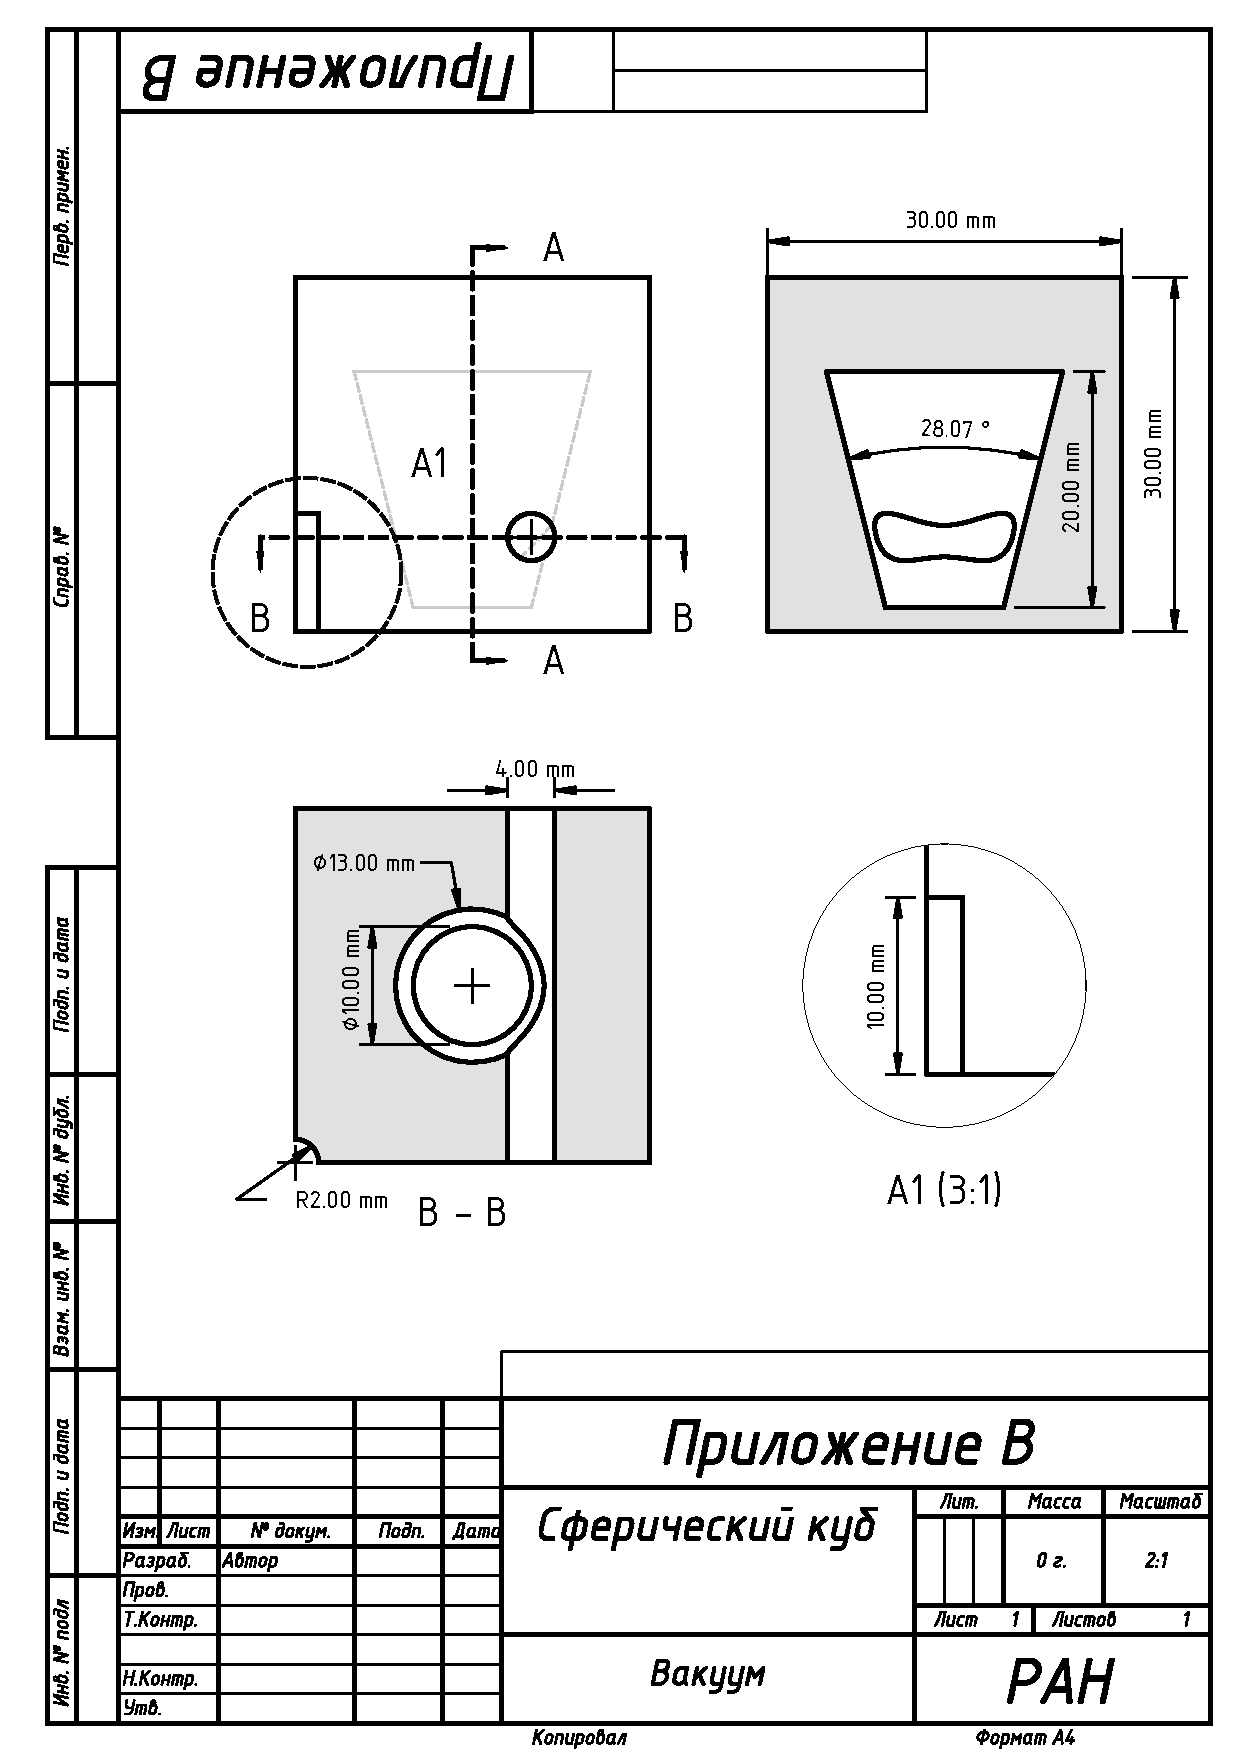
\includepdf[pages=-]{Dissertation/images/drawing.pdf}
